\documentclass[11pt]{article}
\usepackage{geometry}

\geometry{landscape, a4paper, margin=0mm}

\usepackage{amsmath,amssymb}
\usepackage{tikz-qtree}
\usepackage{fullpage}
\usepackage{pdflscape}

\hoffset = 0pt
\voffset = 0pt
\oddsidemargin = -70pt
\topmargin = -70pt
\headheight = 0pt
\headsep = 0pt
\marginparsep = 0pt
\marginparwidth = 0pt
\footskip = 0pt
\textheight = 800pt

\newcommand{\rulefont}[1]{\ensuremath{\mathbf{(#1)}}}

\begin{document}

\pagestyle{empty}

{\footnotesize
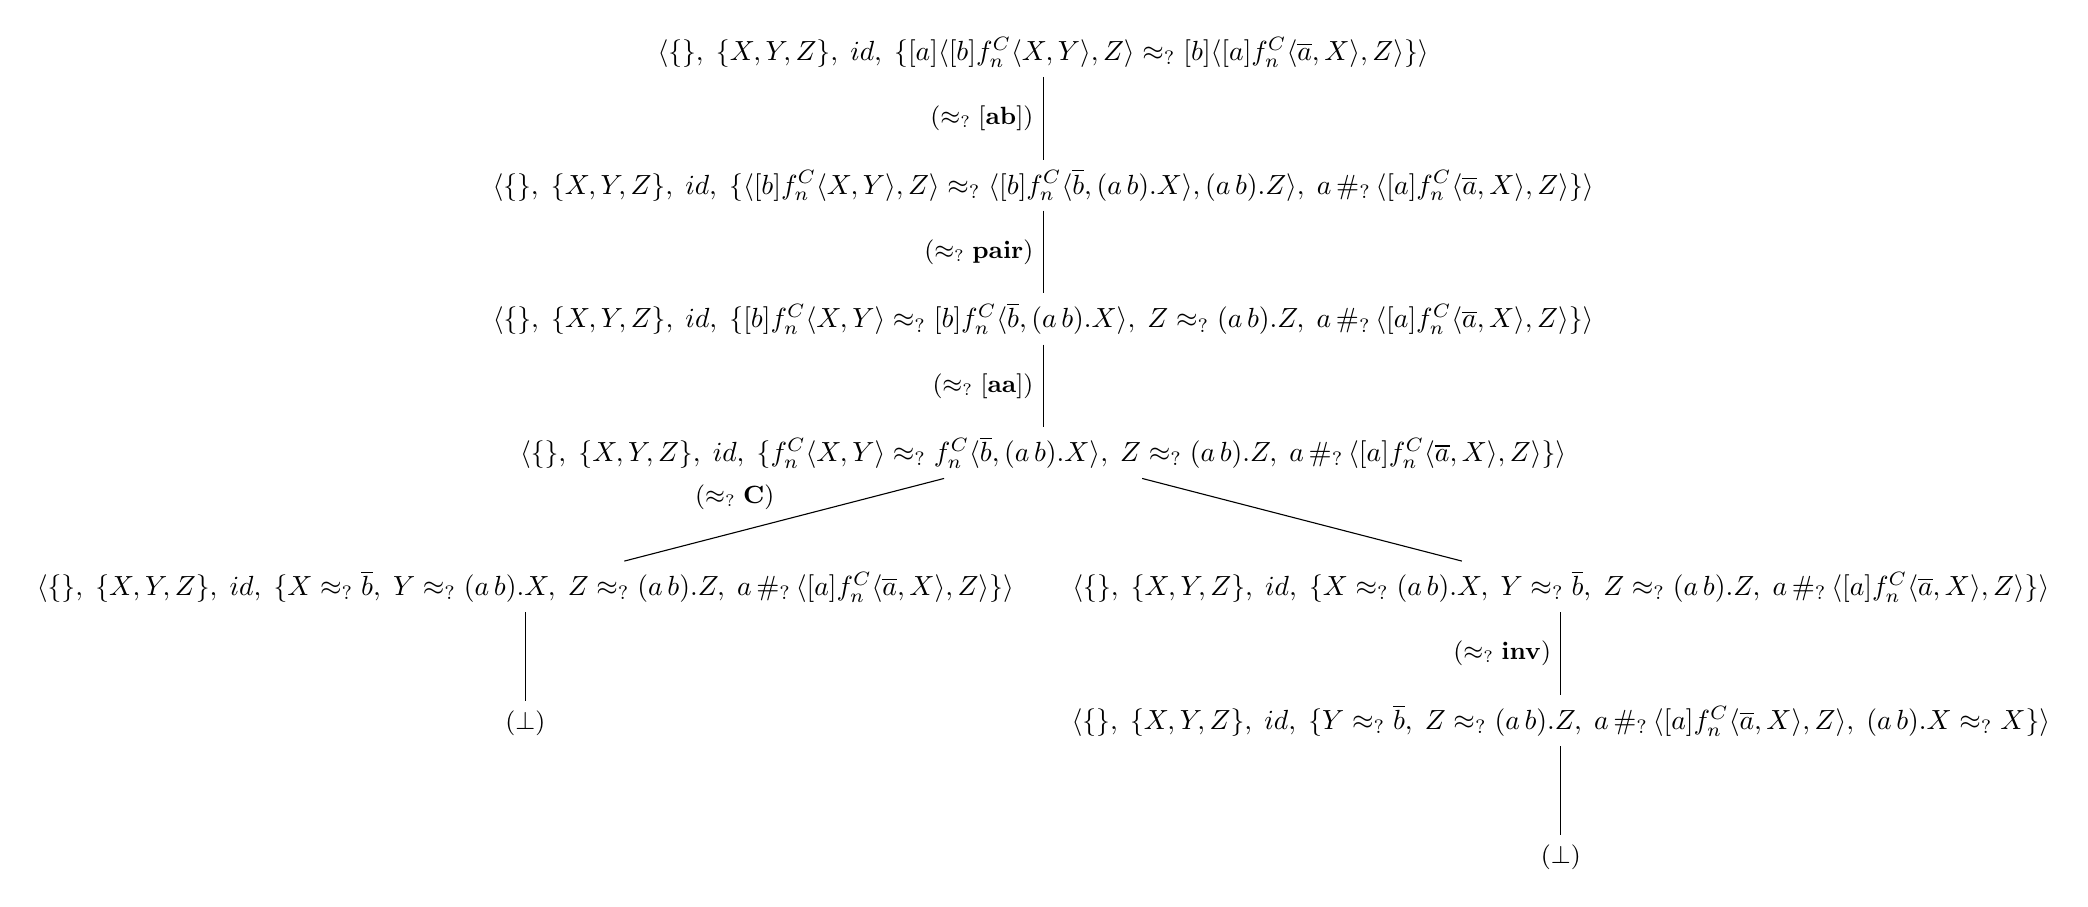
\begin{tikzpicture}[
  level distance=1.7cm,sibling distance=0.5cm,
  edge from parent path={(\tikzparentnode) -- (\tikzchildnode)}]
\tikzstyle{level 1}=[level distance=1.7cm] 
\Tree[.{$\langle\{\}, \;\{X, Y, Z\}, \;id, \;\{[a]\langle [b]f^{C}_{n} \langle X, Y \rangle, Z \rangle\approx_?[b]\langle [a]f^{C}_{n} \langle \overline{a}, X \rangle, Z \rangle\} \rangle$}
	\edge node[auto=right] {\small $\rulefont{\approx_? [ab]}$};
[.{$\langle\{\}, \;\{X, Y, Z\}, \;id, \;\{\langle [b]f^{C}_{n} \langle X, Y \rangle, Z \rangle\approx_?\langle [b]f^{C}_{n} \langle \overline{b}, (a\,b).X \rangle, (a\,b).Z \rangle,\; a\,\#_?\,\langle [a]f^{C}_{n} \langle \overline{a}, X \rangle, Z \rangle\} \rangle$}
	\edge node[auto=right] {\small $\rulefont{\approx_? pair}$};
[.{$\langle\{\}, \;\{X, Y, Z\}, \;id, \;\{[b]f^{C}_{n} \langle X, Y \rangle\approx_?[b]f^{C}_{n} \langle \overline{b}, (a\,b).X \rangle,\; Z\approx_?(a\,b).Z,\; a\,\#_?\,\langle [a]f^{C}_{n} \langle \overline{a}, X \rangle, Z \rangle\} \rangle$}
	\edge node[auto=right] {\small $\rulefont{\approx_? [aa]}$};
[.{$\langle\{\}, \;\{X, Y, Z\}, \;id, \;\{f^{C}_{n} \langle X, Y \rangle\approx_?f^{C}_{n} \langle \overline{b}, (a\,b).X \rangle,\; Z\approx_?(a\,b).Z,\; a\,\#_?\,\langle [a]f^{C}_{n} \langle \overline{a}, X \rangle, Z \rangle\} \rangle$}
	\edge node[auto=right] {\small $\rulefont{\approx_? C}$};
[.{$\langle\{\}, \;\{X, Y, Z\}, \;id, \;\{X\approx_?\overline{b},\; Y\approx_?(a\,b).X,\; Z\approx_?(a\,b).Z,\; a\,\#_?\,\langle [a]f^{C}_{n} \langle \overline{a}, X \rangle, Z \rangle\} \rangle$} [.{\small $\rulefont{\bot}$} ]] [.{$\langle\{\}, \;\{X, Y, Z\}, \;id, \;\{X\approx_?(a\,b).X,\; Y\approx_?\overline{b},\; Z\approx_?(a\,b).Z,\; a\,\#_?\,\langle [a]f^{C}_{n} \langle \overline{a}, X \rangle, Z \rangle\} \rangle$}
	\edge node[auto=right] {\small $\rulefont{\approx_? inv}$};
[.{$\langle\{\}, \;\{X, Y, Z\}, \;id, \;\{Y\approx_?\overline{b},\; Z\approx_?(a\,b).Z,\; a\,\#_?\,\langle [a]f^{C}_{n} \langle \overline{a}, X \rangle, Z \rangle,\; (a\,b).X\approx_?X\} \rangle$} [.{\small $\rulefont{\bot}$} ]]  ]
  ]
  ]
  ]
  ]
\end{tikzpicture}
}

\end{document}
